% !Mode:: "TeX:UTF-8"
\chapter{目标检测与多目标跟踪}
\label{technologies}
本工作主要涉及到目标检测与多目标跟踪领域,相关技术原理比较多。在详细介绍本工作主要内容之前,有必要单独使用一章内容介绍目标检测与多目标跟踪的相关技术原理,为下一章DODT模型的介绍提供技术参考。

\section{目标检测}
\label{object_detection}
目标检测 (Object Detection) 作为计算机视觉中最基本的任务之一,一直以来都受到了学术界与产业界的密切关注。 特别是在最近二十多年,随着深度学习技术的飞速发展, 神经网络已经是目标检测中必不可少的组成部分。 可以说,是深度学习的引入将目标检测推向了新的高度, 使其性能远远超出了传统方法。 以图像数据为例, 目标检测需要在图片中精确找出物体所在的位置 (一般以矩形框出),并标注物体的类别。由于物体的尺寸变化范围很大,摆放物体的角度、姿势等也不确定,并且物体间也会有重叠,这些问题使得目标检测问题并不是那么容易解决。现阶段基于深度学习的目标检测框架主要有两类, 一类是以 Faster-RCNN\cite{ren2015faster} 为代表的两阶段目标检测方法, 另一类是以 YOLO\cite{redmon2016you} 为代表的单阶段目标检测方法。 本小节将详细介绍这两种框架的发展历史、框架结构与实现原理, 此外,本小节也将简单介绍三维目标检测与二维目标检测的差异。

\subsection{两阶段目标检测}
\label{two-stage}
目标检测任务包含目标识别以及目标定位两个子任务, 一般的实现思路是先用区域提取算法截取图像中可能是目标的区域(候选区域),提取特征后分别送入分类器进行分类,以及使用回归算法获得精确的目标边界框(bounding box,bbox)。 先使用一个模块提取候选区域框,然后使用另外的模块完成后续的分类回归任务,这就是两阶段物体检测的实现思路。 两阶段物体检测算法的代表是R-CNN系列工作,该系列历经 R-CNN\cite{6909475},Fast-RCNN\cite{girshick2015fast} 再到 Faster-RCNN\cite{ren2015faster}, 将两阶段物体检测框架不断完善,成为目标检测领域的经典之作。 

\subsubsection{发展历程}

\begin{figure}[!t]
	\centering
	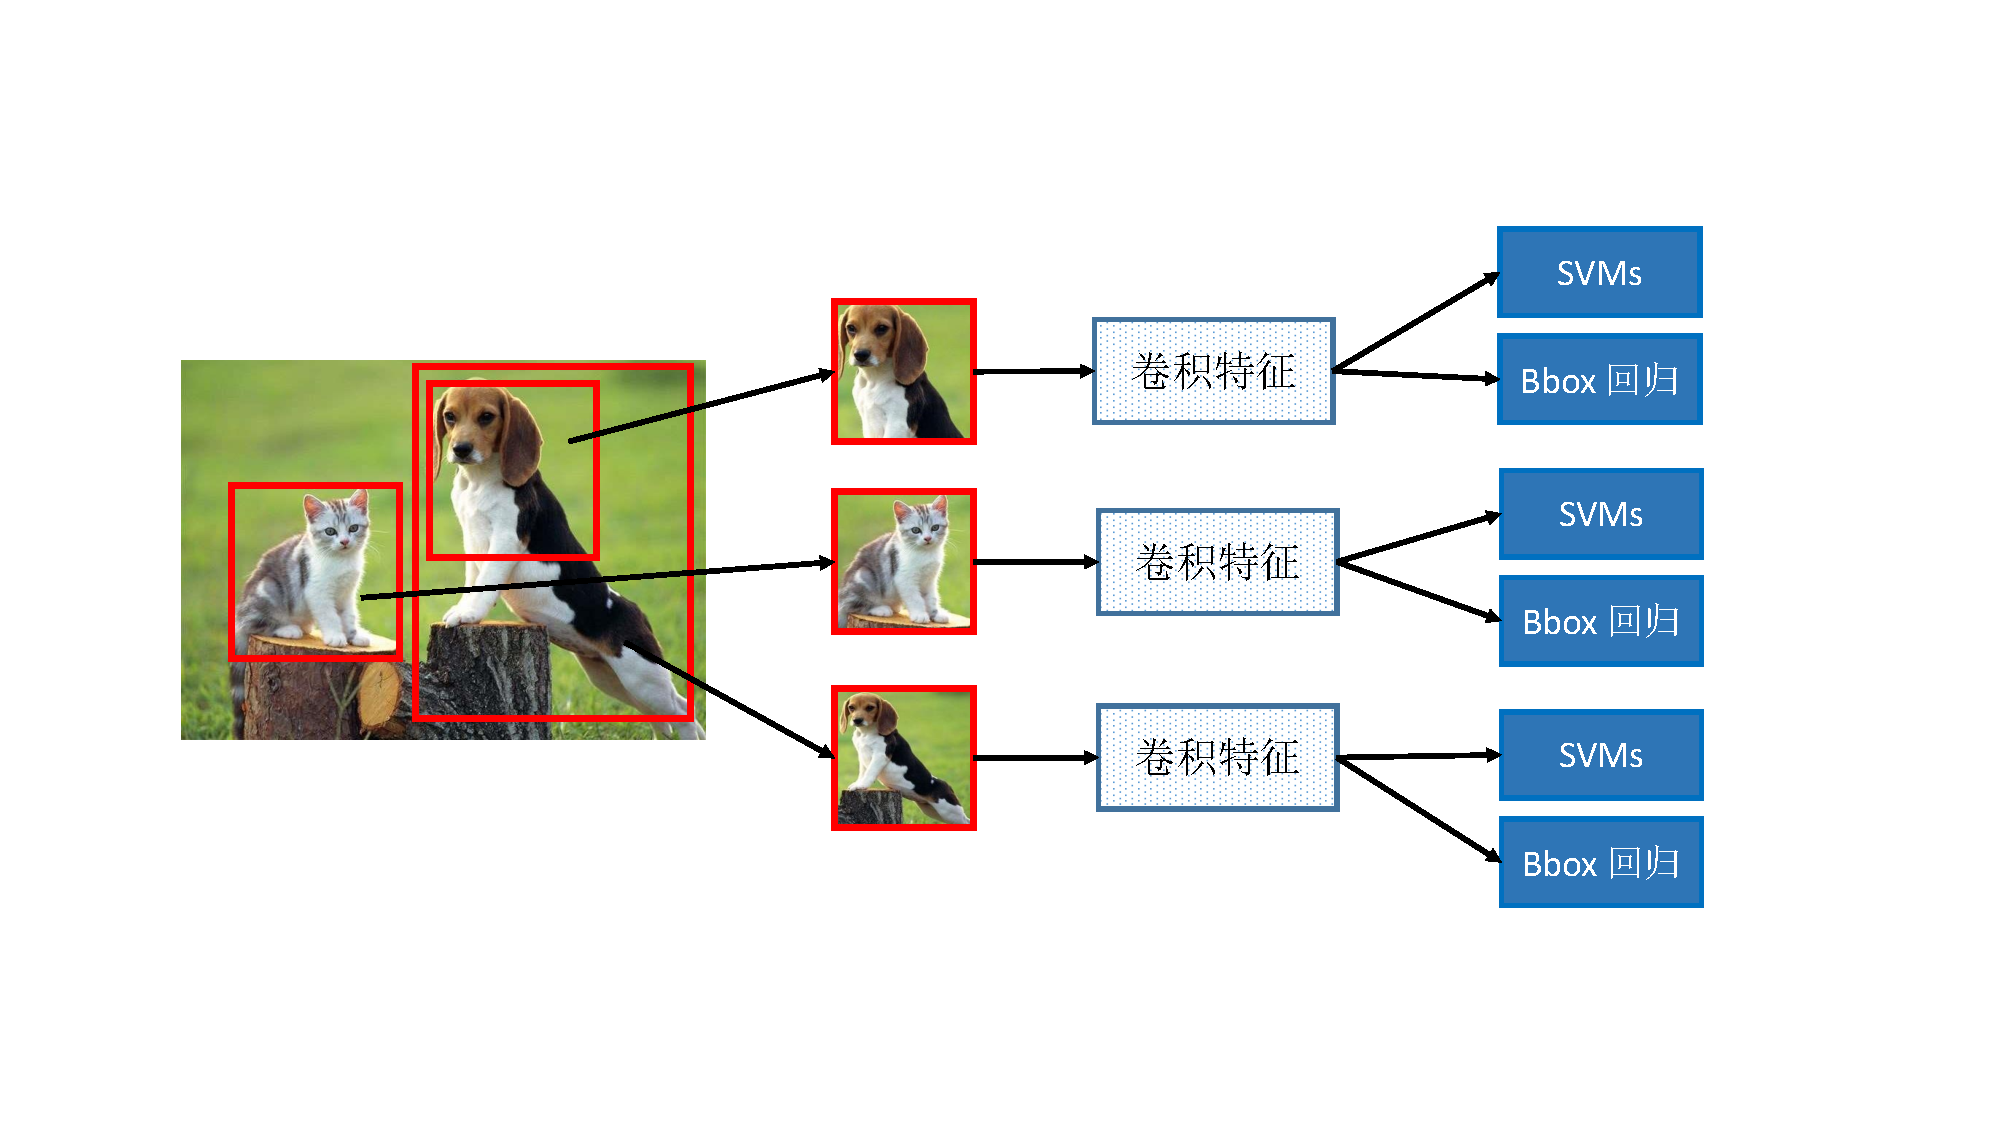
\includegraphics[trim={3cm, 3.5cm, 5cm, 4cm}, clip, width=\textwidth]{./imgs/RCNN.pdf}
	\caption{R-CNN 结构示意图,红框为由选择性搜索算法生成的候选框。}
	\label{fig:rcnn}
\end{figure}

\begin{figure}[!t]
	\centering
	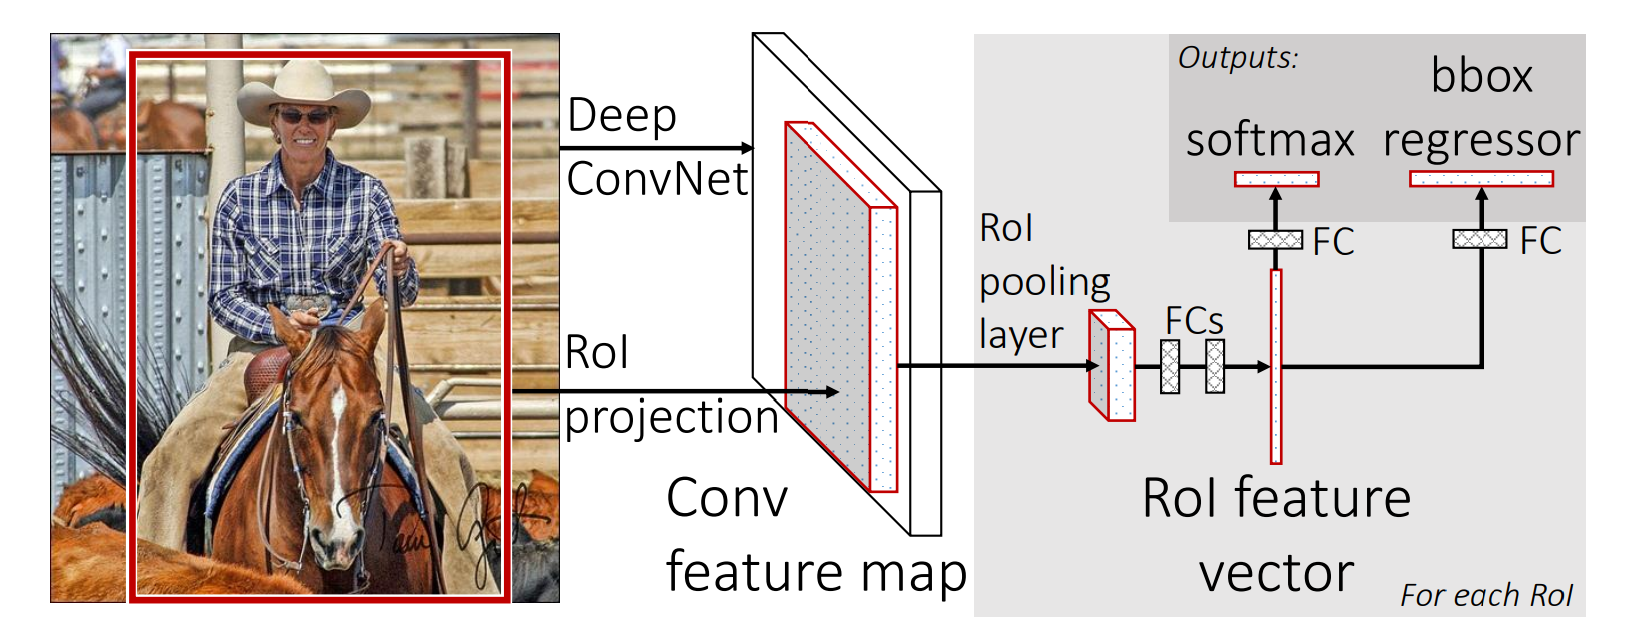
\includegraphics[width=0.95\textwidth]{./imgs/fast-rcnn.png}
	\caption{Fast-RCNN 结构示意}
	\label{fig:fast-rcnn}
\end{figure}


R-CNN可以说是利用深度学习技术进行目标检测的开山之作,其基本结构如图\ref{fig:rcnn}所示。 该工作使用选择性搜索(Selective Search)算法\cite{UijlingsSelective}代替传统的滑动窗口来提取候选区域, 并且利用神经网络对图片进行特征提取,然后利用提取的卷积特征回归更加精确的边界框,同时使用SVMs进行类别判断。该工作奠定了两阶段目标检测框架的基本结构,即一个区域提取(Region Proposal)算法用于提取输入图像中可能是目标的区域, 一个CNN网络用于提取区域特征,一个分类算法用于类别鉴定以及一个回归模型用于回归出精确的物体边界框。2015年,在R-CNN的基础上,RBG(Ross B. Girshick) 又提出了Fast-RCNN算法。该算法借鉴了SPP-Net\cite{7005506}的实现,对R-CNN做了改进,使得检测性能进一步提高,其结构如 \figurename \, \ref{fig:fast-rcnn}所示。具体而言有两个重大改进:(1)将候选区域提取阶段移到了图像特征提取之后,即只对原图做一次卷积,然后在特征图上运行候选区域提取算法得到候选区域特征图,然后将每一个提取的特征块输入RoI(Region of interest)层(结构如图\ref{fig:roi}所示)来将不同尺度的特征图转化为相同维度的密集特征向量,之后送入全连接层进行后续处理;(2)R-CNN训练神经网络提取图像特征,之后用支持向量机进行分类以及用一个回归模型精修边界框。而Fast-RCNN则利用两个全连接层(一个分类分支与一个回归分支) 将分类与回归任务整合到一个模型里联合训练,这为之后的目标检测端对端训练打下了基础。

\begin{figure}[t]
	\centering
	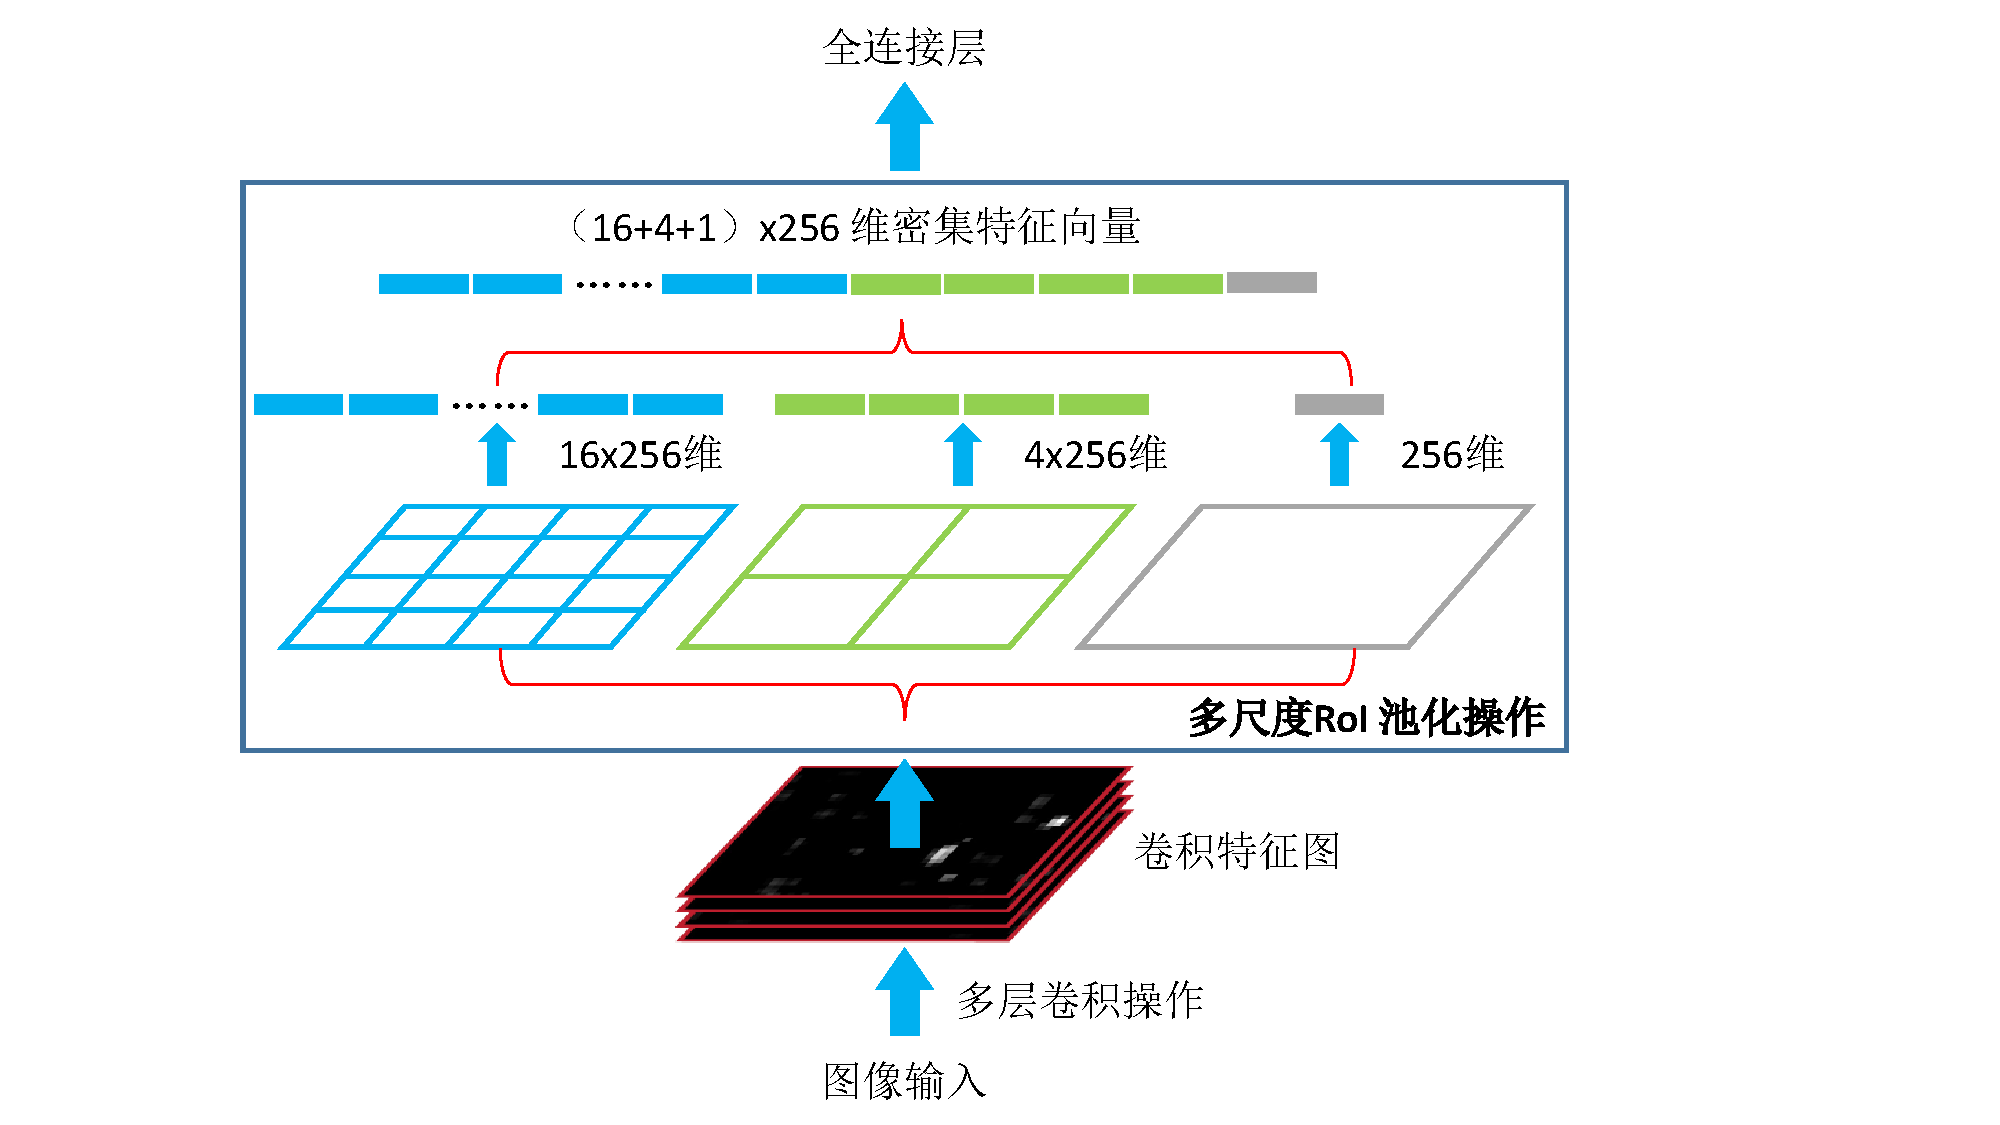
\includegraphics[trim={4cm, 0cm, 7cm, 0cm}, clip,width=0.8\textwidth]{./imgs/roi.pdf}
	\caption{RoI层将不同尺寸的特征图转换为密集特征向量,然后输入全连接层。图中为多尺度RoI池化操作,Fast-RCNN原工作使用的是单尺度,譬如只有4x4的池化操作。}
	\label{fig:roi}
\end{figure}


尽管Fast-RCNN 相对于 R-CNN 已经提速了不少,但要实现实时检测,网络运行速度还是不够,其中主要的瓶颈是候选区域提取阶段十分耗时。基于CPU实现的 Selective Search 算法提取一幅图像的所有候选区域(Proposals)需要约2s时间,效率更高的 EdgeBoxes\cite{Zitnick2014Edge} 算法虽然在一定程度上提高了候选区域提取的准确率和速度,但处理一幅图像仍然需要0.2s。为了解决这个问题,2015年微软亚洲研究院提出了Faster-RCNN算法,该算法引入了候选区域提取网络(Region Proposal Network,RPN),使用神经网络取代传统的区域提取算法,将单幅图像候选区域提取时间缩短到了10ms。下一小节将以Faster-RCNN为代表,重点介绍两阶段物体检测框架的结构以及实现细节。

\subsubsection{Faster-RCNN框架结构}

\begin{figure}[!t]
	\centering
	\begin{minipage}[t]{0.4\textwidth}
		\centering
		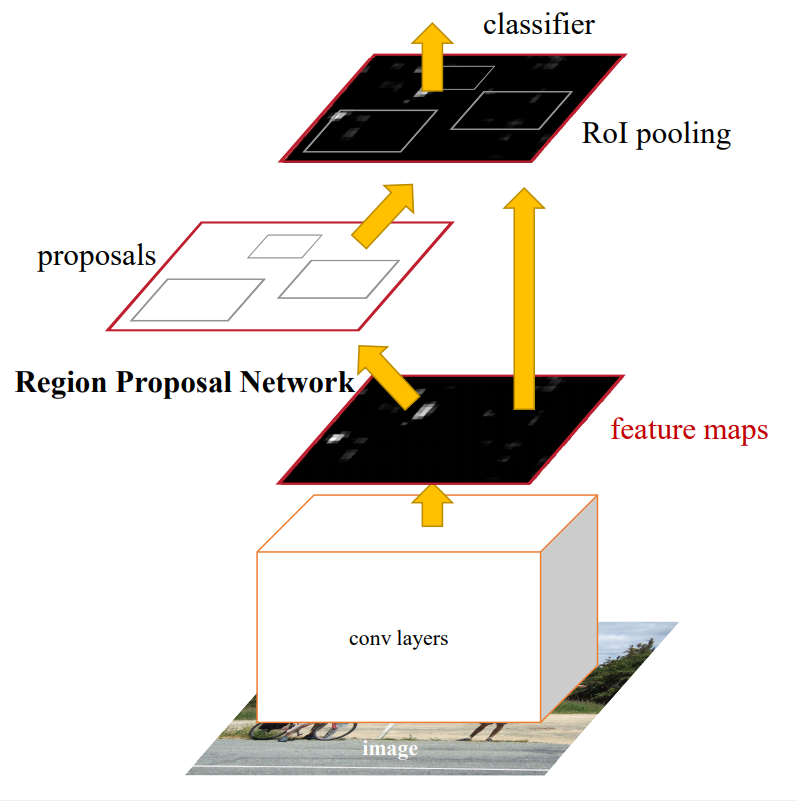
\includegraphics[width=\textwidth]{./imgs/faster-rcnn.png}
		\caption{Faster-RCNN 结构示意}
		\label{fig:faster-rcnn}
	\end{minipage}
	\begin{minipage}[t]{0.58\textwidth}
		\centering
		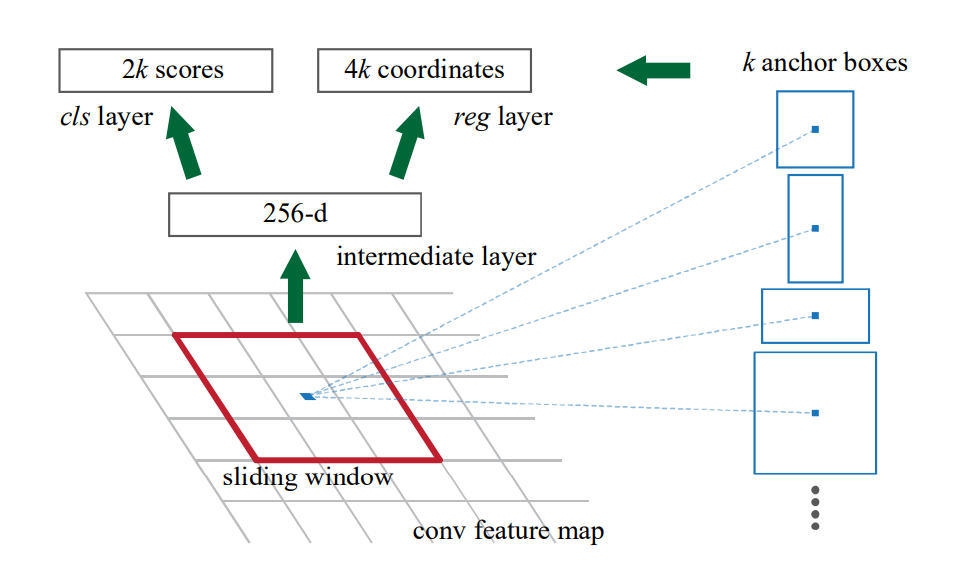
\includegraphics[width=\textwidth]{./imgs/rpn.png}
		\caption{RPN 结构示意}
		\label{fig:rpn}
	\end{minipage}
\end{figure}


Faster-RCNN框架由两大模块组成,候选区域提取模块(RPN)和检测模块, 如 \figurename \, \ref{fig:faster-rcnn} 所示。其中RPN取代了原来的区域提取算法,而检测模块和Fast-RCNN类似,都是由卷积层以及全连接层组成。对于Faster-RCNN网络,首先输入一幅图像,图像经过卷积神经网络提取特征得到卷积特征图(feature maps),然后特征图输入到RPN模块预测得到候选框(proposals),之后根据候选框去特征图中截取相应的特征块。这时的特征块由于尺寸不一样(为了满足物体的尺度多样性,候选框的尺寸不一样),不能直接输入到检测模块进行分类和回归,而是要通过RoI池化操作得到相同尺寸的密集特征向量,然后送入分类分支和回归分支分别预测得到分类结果以及预测框的位置信息。RPN是Faster-RCNN新引进的模块,其原理如\figurename \, \ref{fig:rpn}所示。在特征提取网络生成的特征图($M \times N$)上,使用$k$ 个 $n \times n$ 的卷积核卷积生成$M \times N \times k$个维度为256的中间特征向量,之后输入候选框分类分支和回归分支,分别用来预测候选框的类别(前景/背景,$M \times N \times 2 \times k$)以及候选框的位置信息(中心点坐标$x, y$以及宽高$w, h$, 整体维度为$M \times N \times 4 \times k$)。其中,$k$ 也可以表示为对于特征图上的每一个像素点(或者称为锚点),都负责预测$k$个锚点框(anchor boxes)。另外,为满足候选框的尺寸变化,这$k$个锚点框会设置不同的尺寸和长宽比。原始的Faster-RCNN中设置了三种不同的尺寸:$128\times 128$,$256 \times 256$, $512 \times 512$(px), 也设置了三种不同的长宽比:$1:1$, $1:2$, $2:1$。因此 $k = 3 \times 3 = 9$,意味着每个锚点负责预测9个不同的候选框。

\subsubsection{Faster-RCNN网络训练}
构建好了网络结构,网络的训练还需要准备训练数据,明确损失函数等。目标检测的训练数据一般有公开的数据集,如COCO\footnote[5]{http://cocodataset.org/},PASCAL\footnote[6]{http://host.robots.ox.ac.uk/pascal/VOC/}等,然而Faster-RCNN还需额外训练RPN网络,因此需要额外准备RPN网络训练的标签数据。候选框标签的生成需要借助真实标签数据:首先根据上文提到的锚点的概念,以特征图尺寸为参照生成$M \times N \times k$个候选框(一共有$M \times N$个锚点,每个锚点有$k$个不同尺寸的锚点框),然后根据候选框与真实物体框的重叠程度(一般以候选框与真实框的交并比IoU为量化指标)计算每个候选框的得分。候选框的得分可作为其划分前景类还是背景类的依据,譬如得分大于0.65划分为前景,小于0.35划分为背景,而得分在[0.35,0.65]之间的候选框则忽略不计,这样就得到了训练RPN网络的标签数据。

\begin{figure}[t]
	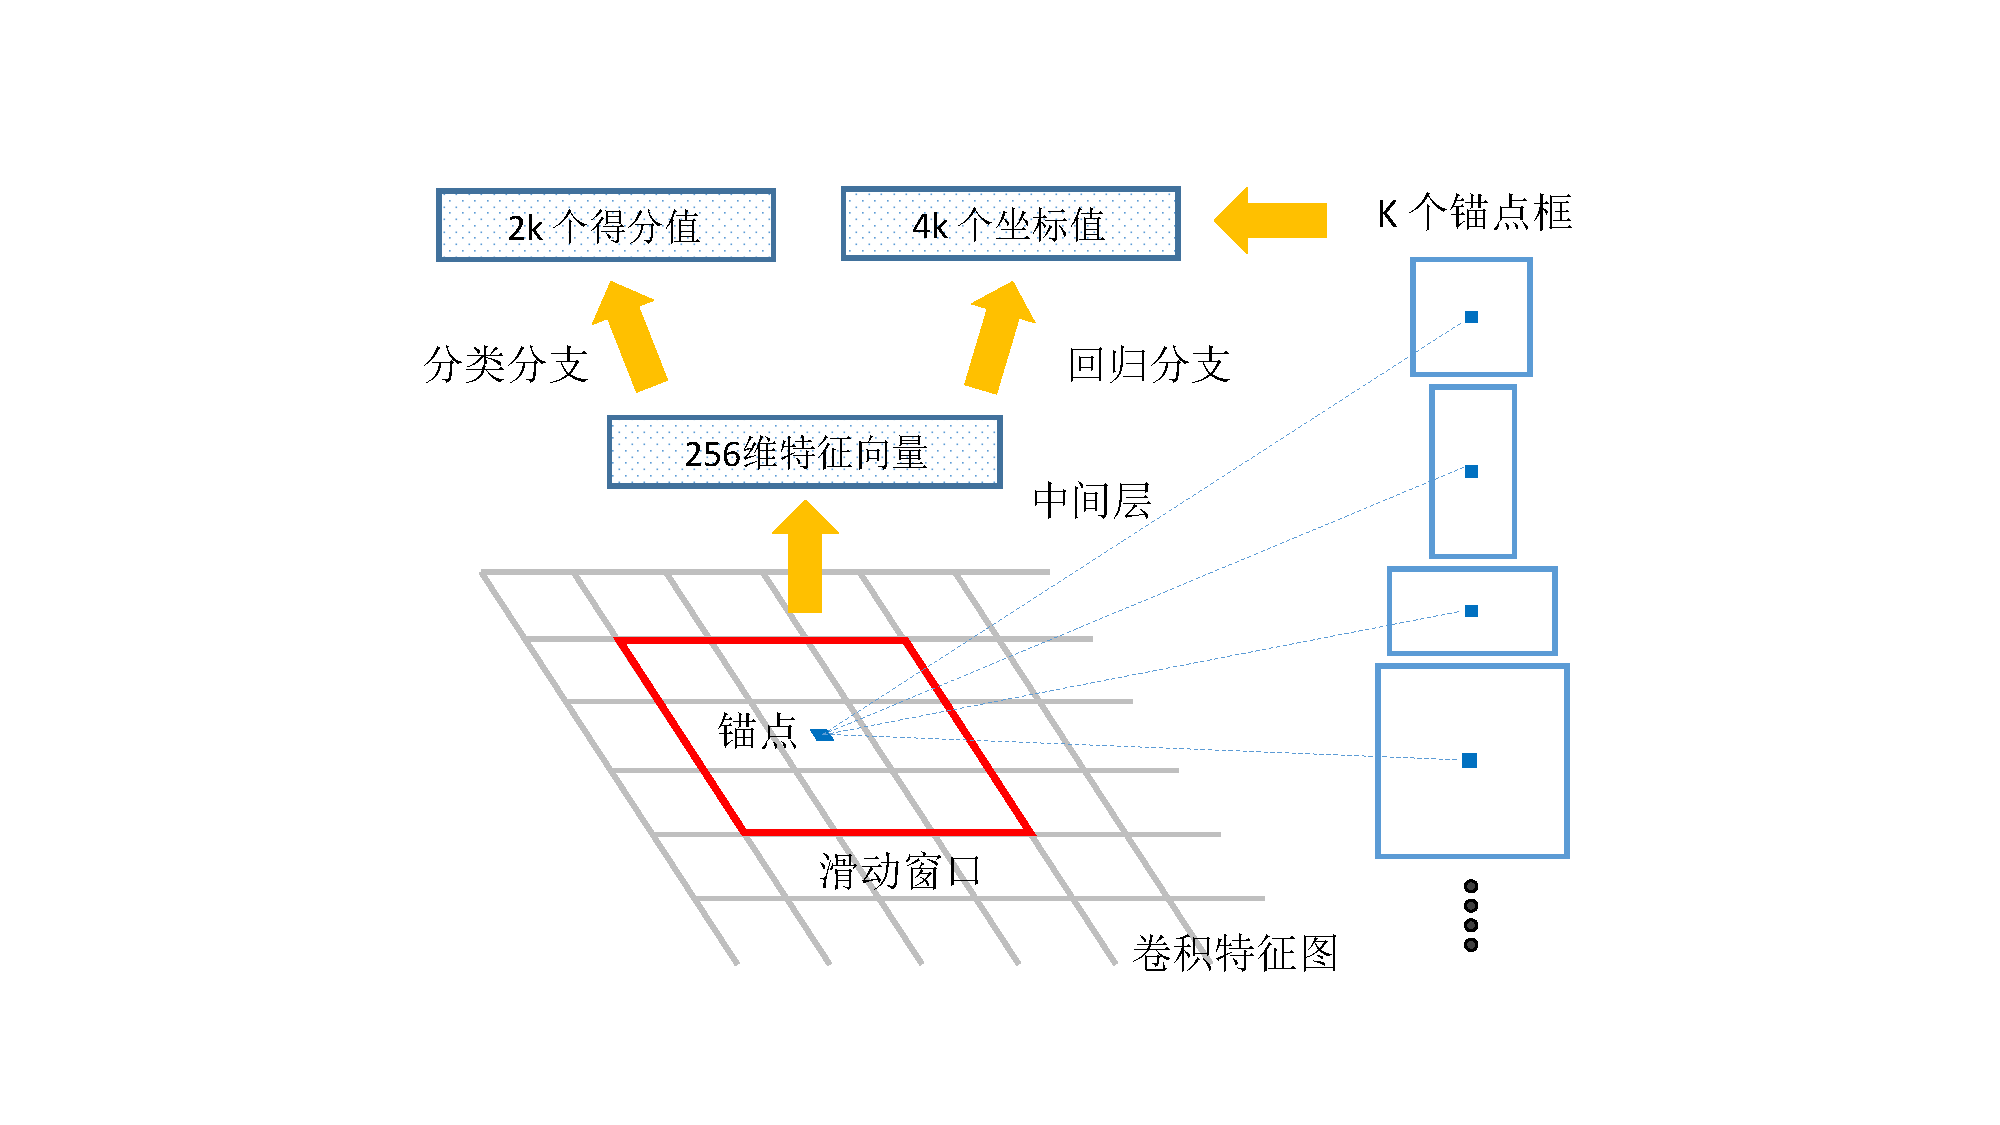
\includegraphics[trim={5cm, 2cm, 5cm, 3cm}, clip,width=0.9\textwidth]{./imgs/rpn.pdf}
	\caption{候选框提取网络结构细节。}
	\label{fig:rpn}
\end{figure}


Faster-RCNN的损失函数由两部分构成,RPN损失和Fast-RCNN损失,并且这两部分损失又都包括两类损失,分类损失和回归损失。
\begin{equation}
L(\{p_i\},\{t_i\}) =\frac{1}{N_{cls}} \sum_{i}L_{cls}(p_i, p^*_i) + \lambda \frac{1}{N_{reg}} \sum_{i} p^*_i L_{reg}(t_i,t^*_i)
\label{con:rpn_loss}
\end{equation}
RPN损失函数如公式 \ref{con:rpn_loss} 所示,其中第一部分为分类损失,第二部分为回归损失。分类损失计算了RPN预测生成的候选框类别的交叉熵损失$L_{cls}$, 其公式如 \ref{con:cross_entropy}所示。其中$p_i$为预测生成的候选框类别,$p^*_i$是标签值。RPN网络生成的候选框分为前景和背景,前景标签为1,背景为0,是一个二分类问题。
\begin{equation}
L_{cls} = -\log[p^*_ip_i + (1-p^*_i)(1-p_i)]
\label{con:cross_entropy}
\end{equation}
在训练中,RPN网络生成的$M \times N \times k$个候选框,然而并不是每个候选框都会纳入损失值的计算范围,因为这些候选框有很多会重叠在一起。Faster-RCNN使用了非极大值抑制(Non-Maximum Suppression,NMS)算法进行初步筛选,减少重叠的候选框。NMS算法详细流程如算法 \ref{alg:nms} 所示:对于RPN生成的候选框集合 $\mathcal{B}$以及对应的置信度集合$\mathcal{S}$,首先选择对应最大置信度的候选框$M$,将其从$\mathcal{B}$中移除并加入最终候选框集合$\mathcal{D}$;然后遍历$\mathcal{B}$,移除与$M$的交并比(Intersection of union, IoU)大于阈值$\epsilon$的框;重复此过程,直到$\mathcal{B}$为空。通过选择合适的阈值(Faster-RCNN中为0.7),NMS算法可以过滤掉大部分重叠的候选框,之后从中随机选取$N_{cls}$个候选框计算分类损失,在Faster-RCNN中$N_{cls} = 256$。
\begin{algorithm}[t]
	\caption{非极大值抑制算法}
	\label{alg:nms}
	\textbf{输入: } $\mathcal{B}=\{b_1,...,b_N\}$,RPN生成候选框集合; $\mathcal{S}=\{s_1,...,s_N\}$, 生成候选框对应的置信度集合; $\epsilon$, 置信度阈值 \\
	\textbf{初始化:} $\mathcal{D} \leftarrow$ \{ \},最终候选框集合 \\
	\While{$\mathcal{B} \neq \emph{empty }$}{
		$m \leftarrow \emph{argmax } \mathcal{S}$ \\
		$\mathcal{M} = b_m$ \\
		$\mathcal{D} \leftarrow \mathcal{D} \bigcup \mathcal{M}; \, \mathcal{B}  \leftarrow\mathcal{B} - \mathcal{M}$ 
	 
		\For{$b_i \emph{ in } \mathcal{B}$}{
			\If{$\emph{IoU}(\mathcal{M},b_i) \leq \epsilon$}{
				$\mathcal{B} \leftarrow \mathcal{B} - b_i; \, \mathcal{S} \leftarrow \mathcal{S} - s_i$
			}
		}
	}
	\textbf{输出: } $\mathcal{D},\mathcal{S}$
\end{algorithm}

RPN回归损失计算预测候选框的$Smooth_{L1}$损失$L_{reg}$,注意到RPN回归损失只计算前景的损失,因此$L_{reg}$前需乘以$p^*_i$(前景为1,背景为0)。$N_{reg} = N_{cls}$,为经过NMS算法过滤后随机选择的候选框数。$Smooth_{L1}$损失公式如\ref{con:smooth_l1}所示,
\begin{equation}
L_{reg}(t_i,t^*_i) = 
\begin{cases}
0.5(t_i-t^*_i)^2 & |t_i-t^*_i| \leq 1 \\
|t_i-t^*_i| - 0.5 & \text{否则}
\end{cases}
\label{con:smooth_l1}
\end{equation}
其中 $t_i$和$t^*_i$分别对应预测候选框以及真实候选框的信息。其中$t_i = (t^x_i, t^y_i,t^w_i,t^h_i)$ 为一四维偏移向量,其计算公式如\ref{con:offsets}所示。其中$(x_a,y_a,w_a,z_a)$分别是对应锚点框中心点坐标以及宽高。从损失值的计算可以看出,RPN并不直接回归出候选框的位置信息,而是回归候选框与对应的锚点框的偏移量,这种处理有利于稳定网络的训练过程,也有利于网络的收敛。
\begin{equation}
t_x = \frac{x - x_{a}}{w_{a}}; \, t_y = \frac{y - y_{a}}{h_{a}}; \,
t_w = \log(\frac{w}{w_{a}}); \, t_h = \log(\frac{h}{h_{a}})
\label{con:offsets}
\end{equation}

检测模块的Fast-RCNN的损失和RPN类似,同样由分类损失和回归损失组成。不过RPN的分类损失是二分类的交叉熵损失,而Fast-RCNN的分类损失是多分类的交叉熵损失,不过将类别标签转化为one-hot向量后并没有本质区别。和RPN类似,Fast-RCNN也不针对所有预测框计算损失,而是先通过更严格的NMS算法(Faster-RCNN中阈值设置为0.3)筛选出一批重叠度低、得分高的预测框,然后随机选择一定数量的预测框进行损失值计算。Fast-RCNN的回归损失基本也和RPN的一致,也不直接回归真实框的位置信息,而是回归物体真实框与锚点框的偏移量,偏移量的编码方式与上文RPN中的类似。

\subsection{单阶段目标检测}
\label{one-stage}
从 R-CNN 到 Fast-RCNN 再到 Faster-RCNN,两阶段目标检测方法一直采用先计算出候选区域然后再在候选区域上提取特征进行分类和回归的算法流程。该模式可以获得很好的检测精度,然而在检测速度上还不是很理想,最好的Faster-RCNN只能达到0.2s一帧的检测速度,离实时检测还有很大差距。单阶段目标检测方法则提供了另一种更为直接的设计思路:不显式计算候选框提取候选区域,而是通过神经网络直接预测物体的位置与类别。该模式的代表工作有YOLO\cite{redmon2016you}系列以及SSD\cite{liu2016ssd},本节以YOLO为例,介绍单阶段目标检测的典型框架结构以及实现原理。


\begin{figure}[!t]
	\centering
	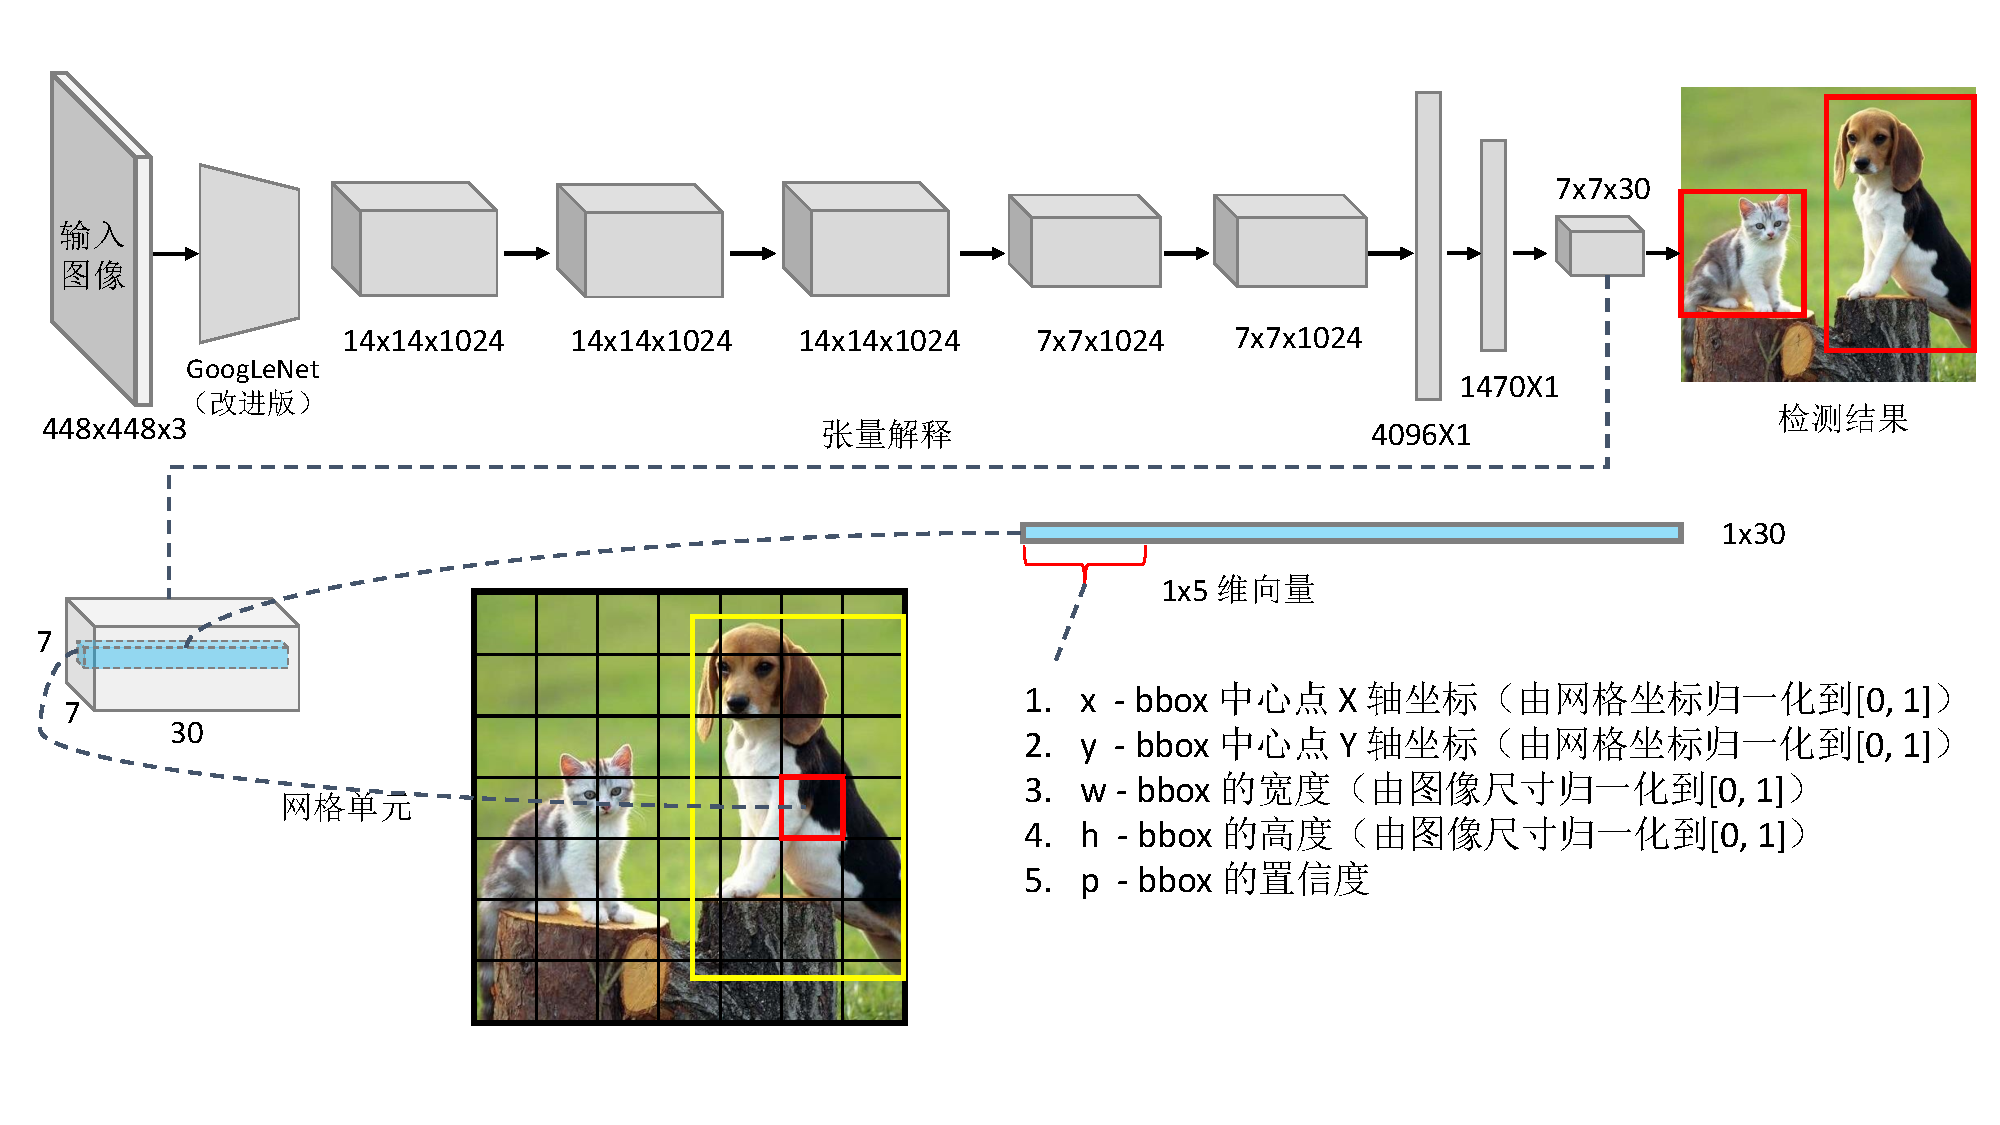
\includegraphics[trim={0.5cm, 2cm, 0cm, 1cm}, clip,width=\textwidth]{./imgs/yolo.pdf}
	\caption{YOLO结构示意图。}
	\label{fig:yolo}
\end{figure}


YOLO的整体架构如\figurename \, \ref{fig:yolo}所示。与R-CNN系列工作不同,YOLO将目标检测任务整体作为一个回归任务来解决。输入一张图像,YOLO首先将输入图像宽高调整到$448 \times 448$,然后输入到由GoogLeNet\cite{7298594,7780677}改进的特征提取卷积网络中,最后输出一个维度为$S \times S \times (B \times 5 + C)$的张量$\mathcal{T}$(YOLO中张量维度为$7 \times 7 \times 30$)。$\mathcal{T}$可以这么理解,首先将一幅图像分成$S \times S$ (YOLO是$7\times 7$)个网格,对于每个网格单元$s$,其对应着$\mathcal{T}$中的一项维度为$1 \times (B \times 5 + C)$的向量$t$。如果一个目标物体的中心落在$s$上,则$s$负责预测该物体,预测结果编码在向量$t$中。$t$维度为$B \times 5 + C$,其中 $B$ 表示每个网格预测$B$个尺度变化的边界框(YOLO中$B=2$);$5$编码了bbox的信息,分别是$(x,y,w,h,c)$,代表bbox中心点坐标、宽高以及置信度;$C$ 表示需要预测$C$个类(YOLO中$C=20$),每个值表示预测为该类的概率值$Pr(class_i|object)$。

和Faster-RCNN类似,YOLO也不是直接回归出物体边界框的实际坐标和宽高,而是bbox相对于单元格的偏移量。对于向量$t=(x,y,w,h,c)$,$(x,y)$的计算公式如\ref{con:yolo_xy}所示,其中$(x_c,y_c)$是bbox中心点的实际坐标,$(w_i, h_i)$是图像的宽高,$x_{col}, y_{col}$是单元格的坐标。最终预测出来的$(x,y)$是经过归一化处理的、中心相对于单元格的偏移。$(w,h)$的计算公式如\ref{con:yolo_wh}所示,是bbox相对于整张图像的比例。置信度$c$的计算公式如\ref{con:yolo_c}所示,由两部分组成,$Pr(object)$表示单元格内是否有物体,有为1,没有则为0;$IoU^{Truth}_{Pred}$表示bbox位置的准确度,用IoU衡量。
\begin{gather}
x = \frac{x_c}{w_i}S - x_{col}; \, y = \frac{y_c}{h_i}S - y_{row} 
\label{con:yolo_xy}\\
w = \frac{w_b}{w_i}; \, h = \frac{h_b}{h_i}
\label{con:yolo_wh}\\
c = Pr(object)*IoU^{Truth}_{Pred}
\label{con:yolo_c}
\end{gather}

在测试阶段,网络最终输出也为一个$S \times S \times (B \times 5 + C)$的张量,其中包含$S \times S \times B$个预测框,每个预测框的最终概率为 $Pr(class_i|object)* c$,综合了定位误差和分类误差。最后这$S \times S \times B $ 列的结果会送入NMS算法去除重复的检测框,得到最终的检测结果。

YOLO的损失函数设计比较复杂,如公式\ref{con:yolo_loss}所示。YOLO的损失函数都采用平方和损失,可分为五部分来看:
\begin{equation}
\begin{split}
L_{yolo} &= \lambda_{coord} \sum^{S^2}_{i=0} \sum^{B}_{j=0} \mathds{1}^{obj}_{i,j} (x_i - \hat{x}_i)^2 + (y_i - \hat{y}_i)^2 \\
&+ \lambda_{coord} \sum^{S^2}_{i=0} \sum^{B}_{j=0} \mathds{1}^{obj}_{i,j} \left(\sqrt{w_i} - \sqrt{\hat{w}_i}\right)^2 + \left(\sqrt{h_i} - \sqrt{\hat{h}_i}\right)^2 \\
&+ \sum^{S^2}_{i=0} \sum^{B}_{j=0} \mathds{1}^{obj}_{i,j}\left(C_i -\hat{C}_i\right)^2\\
&+ \lambda_{noobj} \sum^{S^2}_{i=0} \sum^{B}_{j=0} \mathds{1}^{noobj}_{i,j}\left(C_i -\hat{C}_i\right)^2\\
&+ \sum^{S^2}_{i=0}\mathds{1}^{obj}_{i}\sum_{c \in classes} \left(p_i(c) - \hat{p}_i(c)\right)^2
\end{split}
\label{con:yolo_loss}
\end{equation}
第一部分为bbox中心坐标的误差,其中$\mathds{1}^{obj}_{i,j}$表示判断第$i$个网格中第$j$个bbox是否负责预测该物体。第二部分为bbox宽高的误差,由于在对不同大小的bbox的预测中,小bbox预测偏离的容忍程度比大bbox要小很多,而平方和损失对bbox的尺度并不敏感。为了解决这个问题,YOLO使用宽高的平方根代替原来的宽高。第三部分为含有物体的bbox的置信度预测误差,第四部分为不含物体的bbox的置信度预测误差。最后一部分是对bbox类别预测的误差,其中$\mathds{1}^{obj}_{i}$表示是否有物体落在单元格$i$中。另外,为了平衡各种损失之间的比例,YOLO还加入了$\lambda_{coord}, \lambda_{noobj}$作为超参数平衡各部分损失。

YOLO由于没有显式的预测候选框的过程,因此检测速度很快。但是由于其中网格的划分不可能十分细致,因此YOLO对相互靠的很近的物体(中心可能落在同一个单元格内)、以及小物体检测效果不好。这是由于一个单元格只预测一个类,当物体重叠时,会出现几个不同物体的中心都落在一个单元格的情况。另外,YOLO对于同一类物体出现不常见的长宽比等情况的泛化能力较差,这些问题在其YOLO的后续工作YOLOv2\cite{8100173}、YOLOv3\cite{RedmonYOLOv3}中有探究。

\subsection{三维目标检测}
\label{3d_detection}

\begin{figure}[!t]
	\centering
	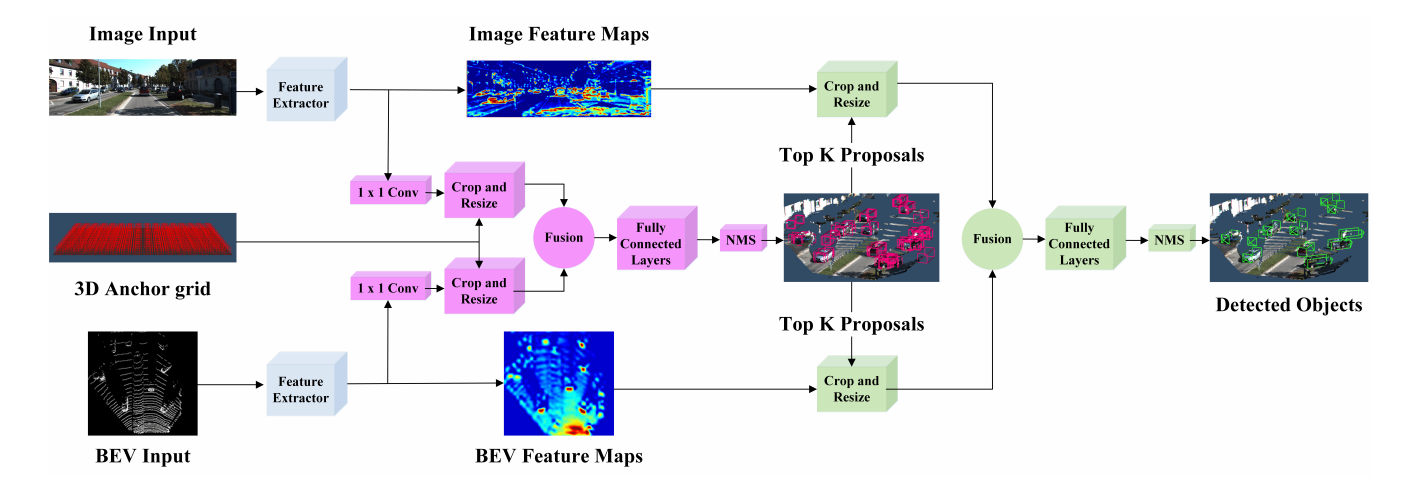
\includegraphics[width=\textwidth]{./imgs/avod.png}
	\caption{AVOD 结构示意图\cite{ku2018joint}。}
	\label{fig:avod}
\end{figure}


三维目标检测任务需要明确目标在三维环境中的位姿状态,包括目标在三维世界的坐标,形状以及朝向。然而,将基于图像的二维目标检测推广到三维对于模型框架本身来说并没有多大变化。以两阶段二维目标检测为例,将其推广到三维空间时,输入数据需要从二维转化到三维,相应的特征提取模块、候选区域提取网络以及结果输出也需要做出调整。两阶段三维目标检测比较有代表性的如AVOD\cite{ku2018joint},网络结构如图\ref{fig:avod}所示。对于特征提取模块,由于AVOD使用的是基于投影的方法编码点云特征,将深度维度转化为通道,和二维RGB图像的特征提取类似,因此不需要做出很大的改变。但是对于其他点云编码方式,可能需要将二维卷积换成三维卷积以完成对三维数据的特征提取。对于RPN模块,AVOD使用的是3D锚点框,提取候选区域特征时是将3D候选框投影到图像以及点云BEV平面,这一点和二维目标检测有很大不同。对于最终的预测框结果输出,AVOD需要输出三维环境下的目标位姿信息,和二维目标检测只需要输出目标中心点坐标以及宽高不同。而在网络训练阶段,损失值的设置也需要将二维框回归的损失转化为三维框回归损失,而对于需要预测目标三维朝向的,还需要加入朝向预测的损失。不过这些损失值的设置基本和二维目标检测类似,这里不做过多介绍。对于单阶段三维物体检测,也需要根据维度的变化对网络结构做出相应的调整,不过整体来说也和二维单阶段目标检测类似。

%对于单阶段三维目标检测,由于不涉及显式的候选框提取网络,因此只需要在数据输入、网格划分以及输出结果设置上调整成三维模式即可。典型的代表有VoxelNet\cite{zhou2018voxelnet},网络结构如图\ref{fig:voxelnet}所示。VoxelNet直接输入三维点云原始数据,并在三维空间中划分网格(体素),让每个非空体素负责预测中心点落入其中的目标。VoxelNet 借鉴了PointNet\cite{qi2017pointnet}中点云特征提取方法,将点云特征编码成了稀疏的四维张量,并通过三维卷积进一步提取特征,最后传入多尺度的候选区域提取模块进一步
%
%\begin{figure}[!t]
	\centering
	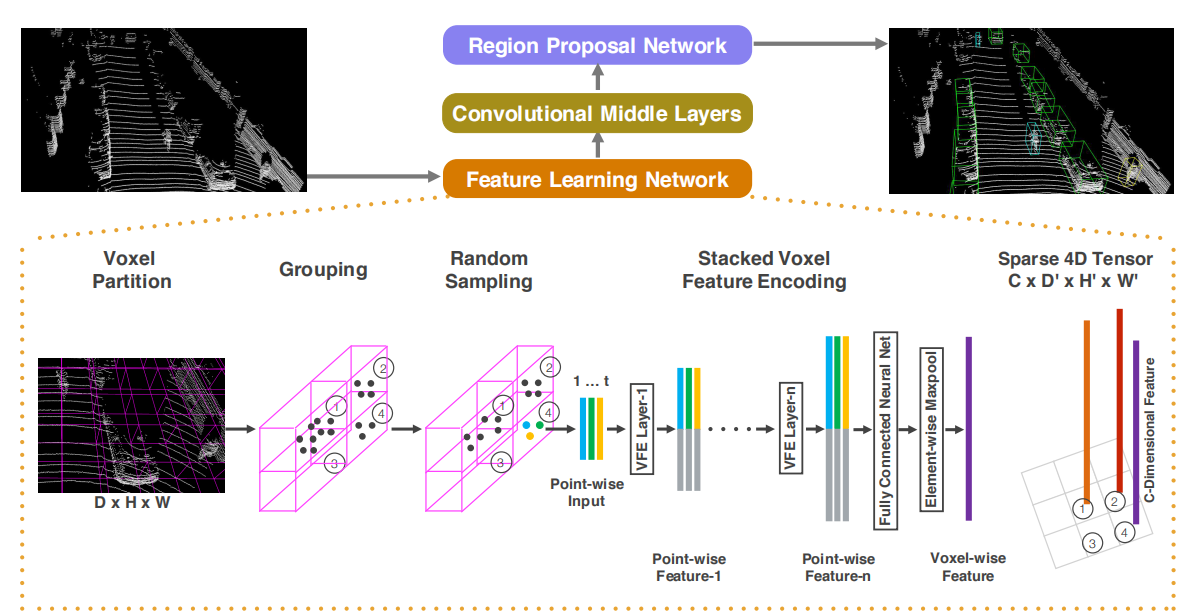
\includegraphics[width=\textwidth]{./imgs/voxelnet.png}
	\caption{VoxelNet 结构示意图\cite{zhou2018voxelnet}。}
	\label{fig:voxelnet}
\end{figure}


\section{目标跟踪}
\label{object_tracking}
由于本工作也涉及到一些目标跟踪方面的应用,因此本章将简单介绍下目标跟踪的一些基本理论。目标跟踪问题是指给定第一帧物体的位置,根据算法预测出后续帧中该物体的位置。根据同时追踪物体的数量的不同,目标追踪分为单目标追踪(Single Object Tracking, SOT)和多目标追踪(Multiple Object Tracking, MOT)。SOT与MOT虽然都属于目标跟踪,但确是两个差别很大的研究方向。由于本工作只涉及到多目标跟踪,因此会重点介绍MOT,而单目标跟踪只会简单叙述其基本原理。

\subsection{单目标跟踪}
\label{single_tracking}

单目标跟踪算法可分为生成式和判别式方法。生成式方法使用模型提取目标的外观特征,然后再最小化跟踪目标与候选目标之间的重构误差来确认目标。这类方法注重目标本身的特征提取,但是忽略了目标与背景的差异,在目标外观发生剧烈变化时容易出现目标漂移或丢失。判别式方法则将目标跟踪看成二元分类问题,通过训练分类模型来将目标区域与背景区分。这类方法可以显著区分背景和目标,因此鲁棒性强,是近几年目标跟踪领域的主流方法\cite{Wang2015Understanding}。

\begin{figure}[t]
	\centering
	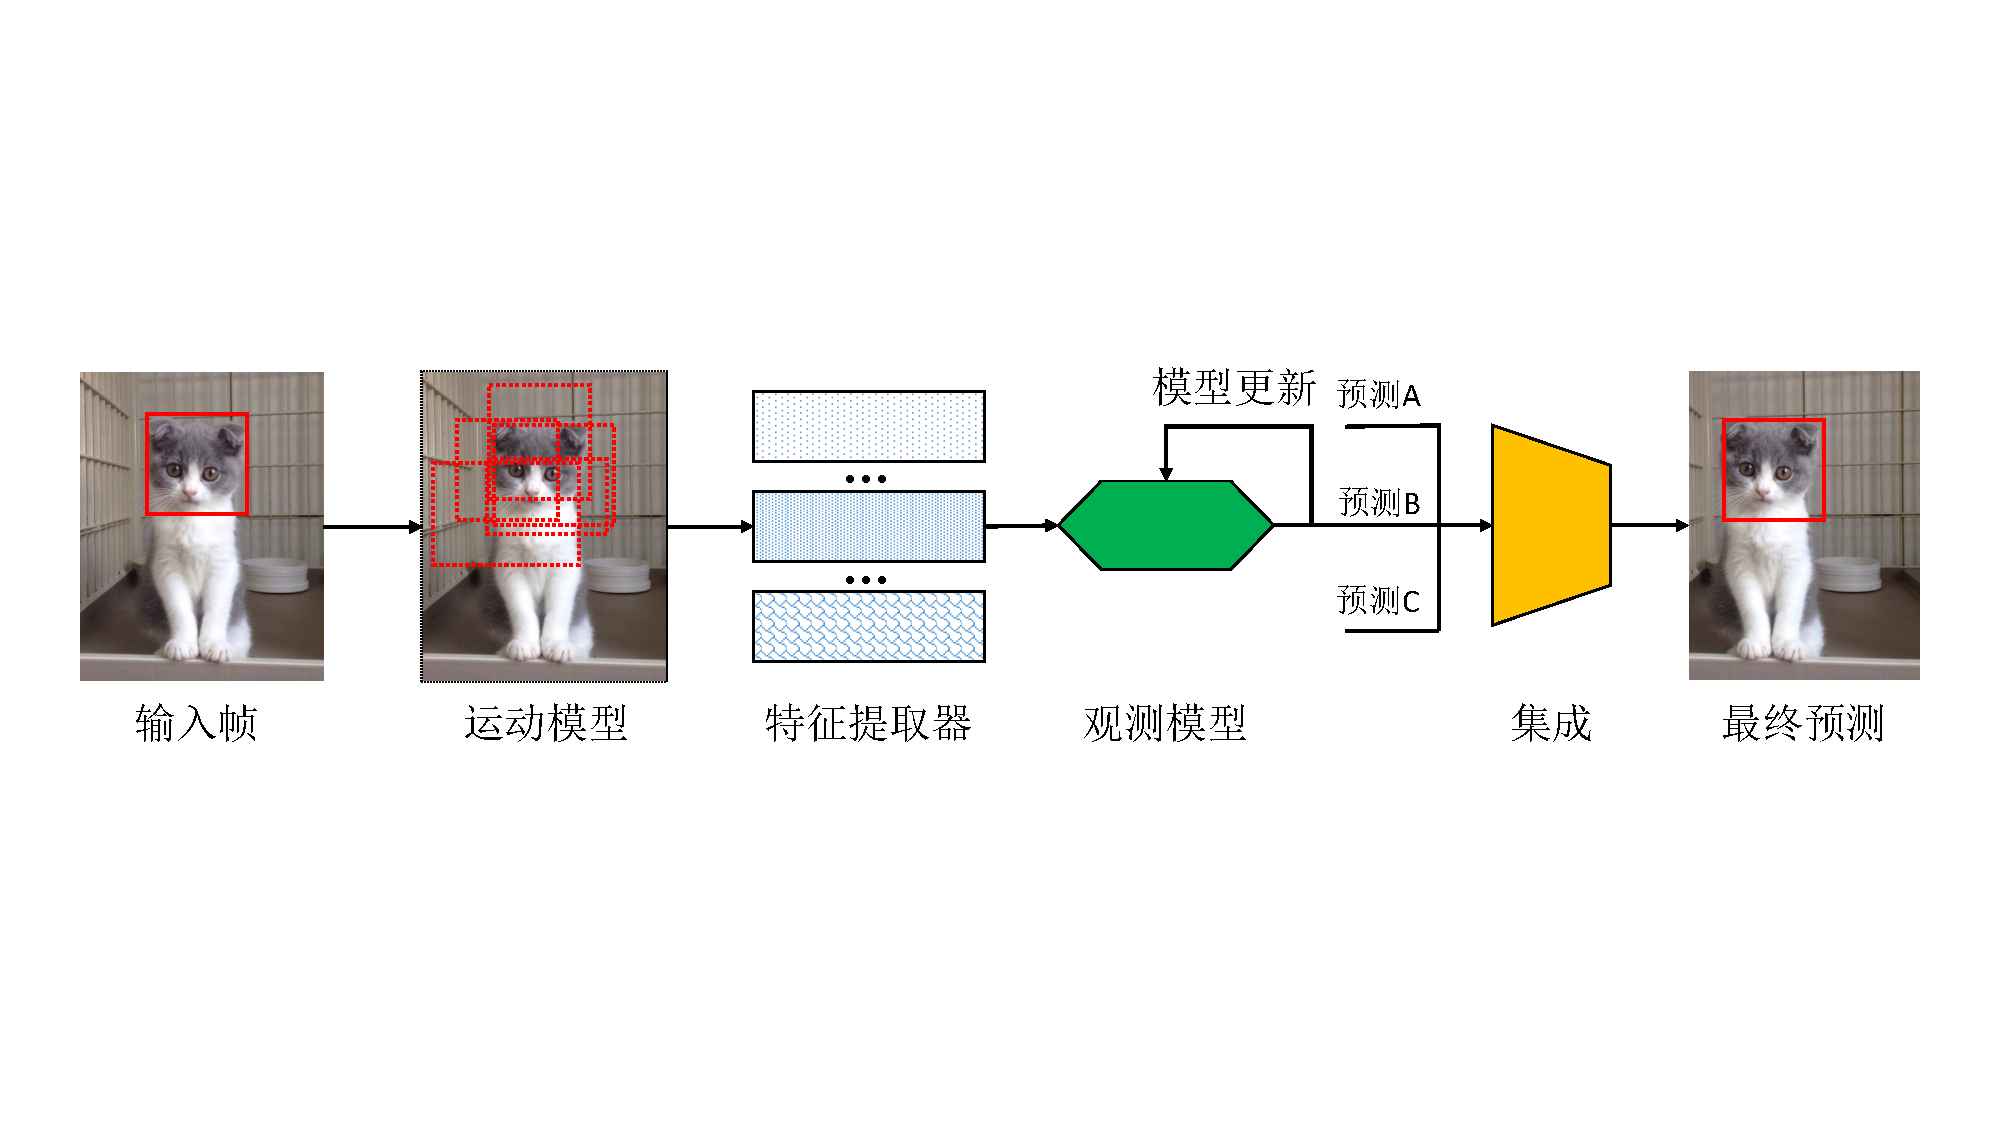
\includegraphics[trim={1cm, 6cm, 1cm, 6cm}, clip,width=\textwidth]{./imgs/sot_pipeline.pdf}
	\caption{单目标追踪流程图。整个流程由四个主要模块组成,分别是运动模块、特征提取模块、观测模块以及模型更新模块。}
	\label{fig:sot_pipeline}
\end{figure}


单目标跟踪算法的基本流程如图\ref{fig:sot_pipeline}所示。输入初始帧并初始化目标框,然后使用\textbf{运动模型}在下一帧中产生众多候选框,之后使用\textbf{特征提取器}提取这些候选框的特征,然后利用\textbf{观测模型}计算这些候选框的置信分数,然后找到最高评分对应的候选框作为预测的目标,或者通过集成方法融合多个候选框以得到更加精确的预测目标。最后,还需要通过\textbf{模型更新器}去更新观测模型。在整个流程中,共涉及到四个主要模块。其中,\textbf{运动模型}的目的是生成众多有效的候选框,其运行速度和质量直接决定了跟踪算法的性能。目前常用的运动模型有粒子滤波以及滑动窗口法。\textbf{特征提取器}决定跟踪系统使用何种特征表征目标,也是目标跟踪的关键。目前常用的特征有手工设计的特征以及使用网络学习的深度特征。其中,手工设计的特征有灰度特征、方向梯度直方图(HOG)、哈尔特征(Haar-like)以及尺度不变特征(SIFT)等。\textbf{观测模型}可分为生成式模型和判别式模型,主要是评价候选框与目标的相似度,目前大多数跟踪方法主要集中在这一块设计。\textbf{模型更新器}需要更新观测模型使其适应目标的变化,防止跟踪过程中发生漂移。

学术界针对单目标追踪有大量的研究,如首次将相关滤波引入单目标跟踪的MOSSE\cite{bolme2010visual}以及后续在此基础上发展的KCF\cite{henriques2014high}、DSST\cite{danelljan2014accurate}、C-COT\cite{danelljan2016beyond}以及ECO\cite{danelljan2017eco}等。另外,这些年基于孪生网络的单目标追踪模型发展迅速,如首先开创端对端深度学习式相关滤波方法先河的SiamFC\cite{bertinetto2016fully},以及加入了RPN应对尺度变化的SiamRPN\cite{li2018high}以及其改进版本DaSiamRPN\cite{zhu2018distractor}等。从近几年的单目标跟踪研究可以看出,深度学习技术也在该领域也引发了技术革新。

\subsection{多目标跟踪}
\label{mot}

相比于单目标跟踪,多目标跟踪问题更加复杂,也更为困难。这是因为多目标跟踪需要考虑流数据中多个独立目标的位置、大小等数据。多个目标各自的外观变化、运动方式的不同、动态光照的影响以及不同目标之间相互遮挡、合并以及分离等情况都是多目标跟踪的难点\cite{Wang2015Understanding}。目前学术界针对多目标跟踪的主流实现思路是基于检测的跟踪(Detection-Based Tracking),该方法要求先由一个目标检测器将每一帧的目标都检测出来,然后再使用框匹配算法将不同帧的同一物体相关联。按照可使用时间帧数据的不同,多目标跟踪算法可分为在线跟踪(Online Tracking)以及离线跟踪(Offline Tracking)。在线跟踪要求算法只能根据当前帧以及之前帧的信息得出下一帧的跟踪结果,而离线跟踪允许算法利用所有帧的信息,获取全局最优解。相对于离线跟踪,在线跟踪更适合实际应用场景。此外,还有一种近似在线跟踪(Near Online Tracking)方法,该方法利用当前帧一定窗口范围内的帧的信息得出下一帧的跟踪结果,是一种折中方法,只会导致些许延迟。

\begin{figure}[t]
	\centering
	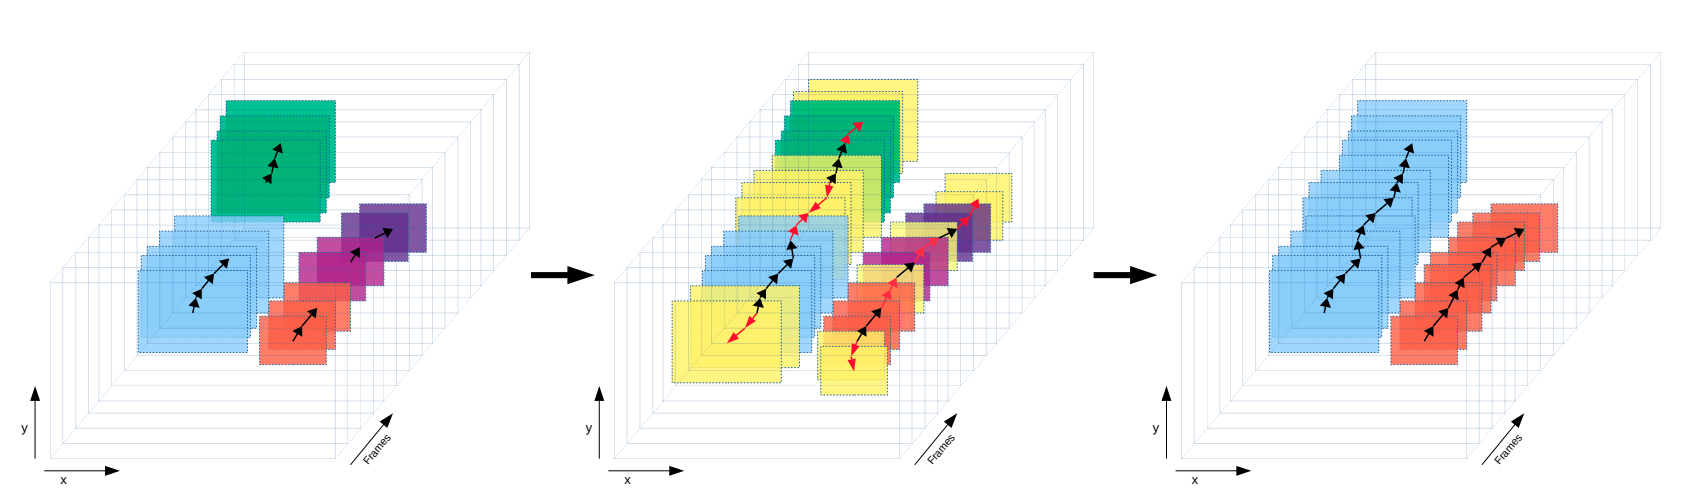
\includegraphics[width=\textwidth]{./imgs/visual_tracking.png}
	\caption{V-IoU Tracker追踪算法基本原理示意图。IoU tracker 方法经常因中间帧的漏检而导致过多的零碎轨迹片段(如左图所示),而这些中间帧的漏检可以通过使用一个视觉追踪模块进行补偿(中间图中黄色框为补偿的漏检框),从而生成片段数更少,连续性更强的轨迹\cite{bochinski2018extending}。}
	\label{fig:visual_tracking}
\end{figure}


目前多目标跟踪算法基本使用现有的检测模型得到所有帧的检测结果,然后设计数据关联算法得到多目标跟踪结果。例如SORT\cite{bewley2016simple}使用Faster-RCNN\cite{ren2015faster}作为目标检测器得到检测结果,然后使用中心坐标、面积、长宽比等对目标运动进行建模,使用卡尔曼滤波预测目标的后续状态,并将预测结果与实际结果进行匹配从而得到最终结果。在此基础上,作者又使用了深度卷积神经网络提取目标特征作为匹配基础改进SORT,从而得到DeepSORT[\cite{wojke2017simple}。此外,还有一种比较简单的,使用前后两帧各目标框的IoU进行关联的匹配算法IoU Tracker\cite{bochinski2017high},该算法严重依赖于检测框的准确率。为了改善对检测结果精度的依赖,作者之后推出了改进版V-IoU Tracker\cite{bochinski2018extending},该算法加入了检测框的长程连续性特征,当前没有检测出新目标的轨迹不再认为立即终止,而是会根据其运动趋势保持更新一定时间步长。如图\ref{fig:visual_tracking}所示,V-IoU Tracker算法通过在原来IoU Tracker算法的基础上增加了一个视觉追踪模块,补偿了中间帧漏检的目标,增加了轨迹的长程连续性。

\begin{algorithm}[!t]
	\caption{改进版 V-IoU Tracker 算法}
	\label{alg:viou-tracker}
	\textbf{输入: }$D=\{D_0,D_1,...,D_{F-1}\} = \{\{d_0, d_1, ..., d_{N_0}\},..., \{d_0, d_1, ..., d_{N_{F-1}}\}\}$\\
	\textbf{初始化:} $T_a=\phi,T_f=\phi, D = \{\{D_i \mid d_i \in D_j, d_j \leq \sigma_{low}\} \mid D_j \in D\}$
	
	\For{$f=0$ to $F$}
	{
		\For{$t_i\in T_a$}
		{
			$d_{best} = d_j$ where $\max(IoU(d_j, t_i)), d_j \in D_f$\\
			\If{$IoU(d_{best},t_i)\geq \sigma_{iou}$}
			{
				使用线性插值生成检测框以替代$t_i$中的虚拟占位框\\
				将$d_{best}$ 添加到 $t_i$,并将 $d_{best}$ 从 $D_f$ 中移除\\
			}
			\ElseIf{$t_i$ 中的虚拟占位框个数小于 $ttl$}{
				将一个新的虚拟占位框添加到$t_i$末尾
			}
			\ElseIf{$highest\_score (t_i) \geq \sigma_{high}$ 并且 $len(t_i)\geq t_{min}$}
			{
				移除$t_i$中的所有虚拟占位框\\
				将 $t_i$ 添加到 $T_f$,并将 $t_i$ 从 $T_a$ 中移除\\
			}
		}
		\For{$d_{j} \in D_f$}
		{
			以$d_j$为起点开始一段新轨迹$t$,并将$t$添加到$T_a$
		}
	}
	\For{$t_j\in T_a$}
	{
		移除$t_j$中的所有虚拟占位框\\
		\If{$highest\_score (t_j) \geq \sigma_{high}$ 并且 $len(t_j)\geq t_{min}$}
		{	
			将 $t_i$ 添加到 $T_f$
		}
	}
	\Return{$T_f$}
\end{algorithm}

V-IoU Tracker算法的具体流程如算法\ref{alg:viou-tracker}所示,其中,$D_f$是当前帧$f$的检测结果集合,$d_j$是$f$中第$j$个检测框,$T_a$为当前还在跟踪的轨迹集合,$T_f$为已经终止的轨迹,$F$是视频序列中帧的总数,$ttl$为允许添加的虚拟占位框的总个数。输入所有帧的检测结果,算法首先过滤掉置信度低于$\sigma_{low}$的检测框,然后对于当前激活的轨迹集合$T_a$中的每一条轨迹$t_i$,如果$t_i$能够根据当前帧找到与其末尾检测框IoU大于$\sigma_{iou}$的预测框,则直接将该预测框添加到$t_i$末尾,并将$t_i$中的虚拟占位框都用插值算法替换为预测框,否则则在$t_i$末尾添加一个虚拟占位框。如果$t_i$中的虚拟占位框个数大于$ttl$,则轨迹$t_i$就被视为已经终止,删除$t_i$中的虚拟占位框,经过轨迹置信度以及长度的筛选后,将其添加到$T_f$中。否则,如果虚拟占位框的个数不超过$ttl$,则继续追踪。虚拟占位框可以补偿由于漏检造成的轨迹中断,从而减少目标跟踪的零碎片段数。本工作的多目标追踪算法借鉴了该思路,只是将2D IoU 计算换成了3D IoU。


多目标跟踪的性能评价指标和单目标跟踪有很大不同,当前学术界最常使用的衡量指标为CLEAR MOT\cite{bernardin2008evaluating}论文提出的多目标追踪准确度(Multiole Object Tracking Accuracy,MOTA)和多目标追踪精确度(Multiple Object Tracking Precision,MOTP)。其中MOTA的计算公式如\ref{con:mota}所示,其中$t$表示帧数,$m_t, fp_t, mme_t$分别是$t$帧时漏检、误检以及错误匹配的数量,$g_t$为$t$帧中的真实标签。从公式可以看出MOTA可以分为三部分,$\overline{m}$为漏检率,$\overline{fp}$为误检率,$\overline{mme}$为错误匹配率,这三种错误率的总和就是总错误率。MOTA直观的给出了衡量算法连续跟踪识别目标的能力,不过没有涉及到目标的检测位置精确度。
\begin{equation}
\begin{split}
MOTA & = 1 - (\overline{m} + \overline{fp} + \overline{mme})\\
& = 1 - \left(\frac{\sum_t m_t}{\sum_t g_t} + \frac{\sum_t fp_t}{\sum_t g_t} + \frac{\sum_t mme_t}{\sum_t g_t} \right)\\
& = 1 - \frac{\sum_t (m_t + fp_t + mme_t)}{\sum_t g_t}
\end{split}
\label{con:mota}
\end{equation}
另一个指标MOTP与MOTA互补,其衡量跟踪目标位置的精确度,而不衡量跟踪识别目标的能力。MOTP的计算公式如\ref{con:motp}所示,其中$t$表示帧数,$i$表示第$t$帧第$i$个目标-预测匹配对,$d^i_t$表示第$t$帧中第$i$个目标-预测匹配对的位置误差,$c_t$表示第$t$帧中总匹配对的个数。在计算MOTA和MOTP时,都是基于整个跟踪过程计算平均值的,而不是基于每一帧的结果,这是因为基于单帧计算然后再求平均会导致和直观上不同的结果。
\begin{equation}
MOTP = \frac{\sum_{i,t} d^i_t}{\sum_t c_t}
\label{con:motp}
\end{equation}

除了MOTA与MOTP,为了更好的在轨迹层面上衡量多目标追踪,学术界一般还会引入其他指标。例如多数追踪率(Mostly Tracked,MT)、多数丢失率(Mostly Lost,ML)、ID切换次数(ID-switches,IDS)、片段数(Fragmentations,FM)。其中MT表示目标的大部分被追踪到的轨迹占比(大于80\%),ML表示目标的大部分跟丢的轨迹占比(小与20\%),IDS为跟踪轨迹改变目标编号的次数,FM为真实轨迹被打断的次数。本工作使用MOTA、MOTP以及以上四种指标评估多目标跟踪算法的性能。

\section{本章总结}
\label{tech_conclusion}
本章主要介绍了本文涉及到的两个领域,目标检测与目标跟踪的基本技术原理。首先介绍了两类目标检测框架的网络结构和训练方法,其中两阶段目标检测以Faster-RCNN作为代表进行介绍,而单阶段目标检测则以YOLO为代表进行介绍。之后,本章简单介绍了单目标跟踪算法的实现思路和几种经典算法。本章最后介绍了多目标跟踪的实现方式和几种典型算法,以及多目标追踪性能的评价指标。该章的内容是为下一章中本工作方法介绍的时候提供技术参考,本章涉及到的技术原理,下章将不再深入介绍。

% 打印时插入必要的空白页
\ifprint
	\newpage
	\thispagestyle{empty}
	\mbox{}
	
	% 避免空白页影响页码编号
	\clearpage
	\setcounter{page}{10}
\fi